\documentclass[%
	final, %
	% draft, % Grafische Elemente durch graue Boxen ersetzen (beschleunigt Kompilieren)
	ngerman,
	% 8pt, % Zu klein, erfordert Paket extsize
	% 9pt, % Zu klein, erfordert Paket extsize
	% 10pt, % für Folien mit sehr viel Text
	% 11pt, % Standardschriftgröße
	 12pt, % etwas größer und daher besser zu lesen
	% 14pt, % deutlich größer, erfordert Paket extsize
	% 17pt, % PowerPoint Standardschriftgröße, erfordert Paket extsize
	% 20pt, % sehr groß, erfordert Paket extsize
	% trans,% Zum Erstellen von Overhead Folien
	% handout, % Erstellen eines Handouts
	% article,% Erstellen eines Artikels
 	% compress, % Die Navigation in der Kopfzeile wird komprimiert dargestellt
	t, % Place text of slides at the (vertical) top of the slides
	% c, % Place text of slides at the (vertical) center of the slides
	% color={}, % list of options for color
	xcolor={table,dvipsnames}, % Optionen für xcolor übergeben
	% hyperref={pdfpagelabels=false}, % list of options for hyperref
	% envcountsect, % Causes theorems, definitions, and so on to be numbered locally to each section.
	% notheorems, % Switches off the definition of default blocks like theorem
	% noamsthm, % Does not load amsthm and also not amsmath
	% ucs, % lädt ucs Paket
	% utf8, % lädt utf8x Paket von ucs (utf8 enconding)
	% dvips, % erzwingt das Laden des dvips Treibers - idR nicht nötig!
	% usepdftitle=false, % Suppresses the automatic generation of title and author entries in the pdf document information.
	% ignorenonframetext, % suppresses content created for the article mode ??
	show notes, % enables Notes
	% leqno,
	% fleqn,
]{beamer}%[2007/03/11] % Minimum necessary version due to severe bugs in version 3.06 !!!
%\let\Tiny=\tiny

% ~~~~~~~~~~~~~~~~~~~~~~~~~~~~~~~~~~~~~~~~~~~~~~~~~~~~~~~~~~~~~~~~~~~~~~~~
% Fonts Fonts Fonts
% ~~~~~~~~~~~~~~~~~~~~~~~~~~~~~~~~~~~~~~~~~~~~~~~~~~~~~~~~~~~~~~~~~~~~~~~~
\usepackage[T1]{fontenc} % T1 Schrift Encoding
\usepackage{textcomp}	 % additional symbols (Text Companion font extension)


% \usepackage{lmodern}               %% --- Latin Modern
\usepackage{mathptmx}              %% --- Times mit Matheschriften
% \usepackage{mathpazo}              %% --- Palantino
% \usepackage{charter}               %% --- Charter
% \usepackage{bookman}               %% Bookman (lädt Avant Garde !!)
% \usepackage{newcent}               %% New Century Schoolbook (lädt Avant Garde !!)

% \usepackage{bera}
\usepackage[scaled=.90]{helvet}    %% --- Helvetica (Arial)
% \usepackage{cmbright}              %% --- CM-Bright (eigntlich eine Familie)
% \usepackage{tpslifonts}            %% --- (Font for Slides)
% \usepackage{avant}      	          %% --- Avantgard
%
\usepackage{courier}               %% --- Courier
%\usepackage[scaled=0.9]{luximono}  	 %% --- Luxi Mono


%%% ===== Sans Serif (kommerzielle Schriften) ============================

% \usepackage[scaled=0.90]{frutiger}  %% --- Adobe Frutiger
% \usepackage[scaled=0.94]{futura}    %% --- Adobe Futura (=Linotype FuturaLT) : Sans Serif
% \usepackage{gillsans}               %% --- Adobe Gill Sans : Sans Serif
% \renewcommand{\sfdefault}{pmy}      %% -- Adobe Myriad  : Sans Serif
% \usepackage[scaled]{asyntax}        %% --- Syntax : sans serif font
% \usepackage[medium]{optima}         %% --- Adobe Optima : Semi Sans Serif
% \renewcommand{\sfdefault}{lo9}      %% --- Linotype ITC Officina Sans

%% ===== Serifen (kommerzielle Schriften ) ================================

% \renewcommand{\rmdefault}{pasx}     %% --- Adobe Aldus
% \usepackage[scaled=1.05]{xagaramon} %% --- Adobe Garamond
% \renewcommand{\rmdefault}{pegx}     %% --- Adobe Stempel Garamond
% \renewcommand{\rmdefault}{pml}      %% --- Adobe Melior
% \renewcommand{\rmdefault}{pmnx}     %% --- Adobe Minion
% \renewcommand{\rmdefault}{psbx}     %% --- Adobe Sabon
% \renewcommand{\rmdefault}{lch}      %% --- Linotype ITC Charter
% \renewcommand{\rmdefault}{lmd}      %% --- Linotype Meridien

% *** Sprache *****************************
\usepackage[ngerman]{babel}
\usepackage[ansinew]{inputenc}
%------------------------------------------

%%% Doc: ftp://tug.ctan.org/pub/tex-archive/macros/latex/required/graphics/grfguide.pdf
% Bilder
\usepackage[%
   %final,
   %draft % do not include images (faster)
]{graphicx}
\usepackage{wrapfig}

%%% Emulationspakete
% \usepackage{beamerprosper}
% \usepackage{beamerseminar}
% \usepackage{beamerfoils}
% \usepackage{beamertexpower}


%%% 4.6.2    Printing the Handout
% \usepackage{pgfpages}
% \pgfpagelayout{resize}[a4paper,border shrink=5mm,landscape]
%     This says “Resize all pages to landscape A4 pages, no what their original size was, but shrink the pages
% by 5mm, so that there is a bit of a border around everything.” Naturally, instead of a4paper you can also use
% letterpaper or any of the other standard paper sizes. For further options and details see the documentation
% of pgfpages.
% \pgfpagelayout{2 on 1}[a4paper,border shrink=5mm]

 \usepackage{movie15}
% \usepackage{multimedia}
%     A stand-alone package that implements several commands for including external animation and sound
%     files in a pdf document. The package can be used together with both dvips plus ps2pdf and pdflatex,
%     though the special sound support is available only in pdflatex.



%% sonstige Pakete ========================
%
% \usepackage{enumitem}
% \usepackage{units}
% \usepackage{pifont}
% \usepackage{subscript}
% -----------------------------------------

\usepackage{tabularx}   % Erweiterte Tabellen Optionen
\usepackage{booktabs}
\usepackage{multicol}


%% Literaturverzeichnis %%%%%%%%%%%%%%%%%%%%%%%%%%%%%%%%%%%%%%%%%%%%%%%
\usepackage[numbers,square]{natbib}
%\bibliographystyle{natdin}
\bibliographystyle{plain}
%%%%%%%%%%%%%%%%%%%%%%%%%%%%%%%%%%%%%%%%%%%%%%%%%%%%%%%%%%%%%%%%%%%%%%%




% *****************************************
% >>> Themes <<<<<<<<<<<<<<<<<<<<<<<<<<<<<<
% *****************************************

% \usetheme[<options>]{<name list>} 		Installs the presentation theme named <name>.
% \usecolortheme[<options>]{<name list>} Same as \usetheme, only for color themes.
% \usefonttheme[<options>]{<name>} 		Same as \usetheme, only for font themes.
% \useinnertheme[<options>]{<name>}		Same as \usetheme, only for inner themes.
% \useoutertheme[<options>]{<name>}		Same as \usetheme, only for outer themes.

% *****************************************
% >>> Themes ohne Navigation
% *****************************************
% \usetheme{default}
% -------------------------------
% \usetheme[]{Bergen}
% -------------------------------
% \usetheme[%
% 	secheader % section im Header
% ]{Boadilla}
% -------------------------------
% % Wie das Boadilla theme, mit kraeftigeren Farben
% % und unveraenderten Icons
% \usetheme[%
% 	secheader % section im Header
% ]{Madrid}
% -------------------------------
% \usetheme{Pittsburgh}
% -------------------------------
% \usetheme[]{Rochester}


% *****************************************
% >>> Themes mit Navigation (Baumstruktur)
% *****************************************
% \usetheme{Antibes}      % flach
% -------------------------------
% \usetheme{JuanLesPins}  % 3D, Schatten
% -------------------------------
% \usetheme{Montpellier}    % flach, wenig Farben


% *****************************************
% >>> Themes mit Navigation (Sidebar)
% *****************************************
% % flach, starke Farben
% \usetheme[%
%  	left, % sidebar links
% % 	right, % sidebar rechts
% % 	hideallsubsections, % nur sections werden angezeigt
% % 	hideothersubsections, % nur subsections der aktuellen section werden angezeigt
% ]{Berkeley}
% -------------------------------
% % wie Berkeley, 3D, starke Farben
% \usetheme[%
%  	left, % sidebar links
% % 	right, % sidebar rechts
% % 	hideallsubsections, % nur sections werden angezeigt
% % 	hideothersubsections, % nur subsections der aktuellen section werden angezeigt
% ]{PaloAlto}
% -------------------------------
% % flach, schwache Farben
% \usetheme[%
%  	left, % sidebar links
% % 	right, % sidebar rechts
% % 	hideallsubsections, % nur sections werden angezeigt
% % 	hideothersubsections, % nur subsections der aktuellen section werden angezeigt
% ]{Goettingen}
% -------------------------------
% % wie Goettingen, flach, starke Farben
% \usetheme[%
%  	left, % sidebar links
% % 	right, % sidebar rechts
% % 	hideallsubsections, % nur sections werden angezeigt
% % 	hideothersubsections, % nur subsections der aktuellen section werden angezeigt
% ]{Marburg}
% -------------------------------
% flach, schwache Farben
% \usetheme[%
% % 	hideallsubsections, % nur sections werden angezeigt
% % 	hideothersubsections, % nur subsections der aktuellen section werden angezeigt
% ]{Hannover}


% *****************************************
% >>> Themes mit Navigation (Mini Frame Navigation)
% *****************************************
% % starke Farben, flach
% \usetheme[
% % 	compress, % Navigation in einer Zeile
% ]{Berlin}
% -------------------------------
% % wie Berlin, runde Kanten, starke Farben, flach
% \usetheme[
% 	compress, % Navigation in einer Zeile
% ]{Ilmenau}
% -------------------------------
% % wie Berlin, starke Farben, flach
% \usetheme[
% 	compress, % Navigation in einer Zeile
% ]{Dresden}
% -------------------------------
% % starke Farben, 3D
% \usetheme{Darmstadt}
% -------------------------------
% % wie Darmstadt, ohne subsections
% \usetheme{Frankfurt}
% -------------------------------
% % flach, schwache Farben
% \usetheme{Singapore}
% -------------------------------
% % flach, horiz. Linien
% \usetheme{Szeged}


% *****************************************
% >>> Themes mit Navigation (Section and Subsection Tables)
% *****************************************
% % flach, rund, starke Farben
% \usetheme{Copenhagen}
% -------------------------------
% % flach, eckig, starke Farben
% \usetheme{Luebeck}
% -------------------------------
% % flach, starke Farben
% \usetheme{Malmoe}
% -------------------------------
% 3D, starke Farben
\usetheme{Warsaw}


% *****************************************
% >>>> 15.1    Inner Themes
% *****************************************
% An inner theme installs templates that dictate how the following elements are typeset:
%    - Title and part pages.
%    - Itemize environments.
%    - Enumerate environments.
%    - Description environments.
%    - Block environments.
%    - Theorem and proof environments.
%    - Figures and tables.
%    - Footnotes.
%    - Bibliography entries.


% >>>  Itemize Bullets
% -------------------------------
% \useinnertheme{default} % Zahlen
% -------------------------------
% \useinnertheme{circles} % Kreise
% -------------------------------
\useinnertheme{rectangles} % Vierecke
% -------------------------------
% \useinnertheme[%
% 	shadow % mit Schatten
% ]{rounded} % 3D Kugeln
% -------------------------------
% \useinnertheme{inmargin} % Bullts im Margin


% *****************************************
% >>>> 15.2    Outer Themes
% *****************************************
% An outer theme dictates (roughly) the overall layout of frames. It specifies where any navigational elements
% should go (like a mini table of contents or navigational mini frames) and what they should look like. Typically,
% an outer theme specifies how the following elements are rendered:
%    - The head- and footline.
%    - The sidebars.
%    - The logo.
%    - The frame title.

% \useoutertheme{default}
% -------------------------------
% \useoutertheme{infolines}
% -------------------------------
% \useoutertheme[%
% 	footline=empty, % suppressed the footline (default).
% % 	footline=authorinstitute, %shows the author's name and the institute in the footline.
% % 	footline=authortitle, % shows the author's name and the title in the footline.
% % 	footline=institutetitle, % shows the institute and the title in the footline.
% % 	footline=authorinstitutetitle, % shows the author's name, the institute, and the title in the footline.

% ]{miniframes}
% -------------------------------
% \useoutertheme[%
% % 	subsection= true,  % or false shows or suppresses line showing the subsection in the headline.
% ]{smoothbars}
% -------------------------------
% \useoutertheme[%
%  	left, % sidebar links
% % 	right, % sidebar rechts
% % 	hideallsubsections, % nur sections werden angezeigt
% % 	hideothersubsections, % nur subsections der aktuellen section werden angezeigt
% ]{sidebar}
% -------------------------------
% % This theme installs a headline in which, on the left, the sections of the talk are shown and, on the right,
% % the subsections of the current section. If the class option compress has been given, the sections and
% % subsections will be put in one line; normally there is one line per section or subsection.
% \useoutertheme{split}
% The colors are taken from palette primary and palette fourth.
% -------------------------------
% % This layout theme extends the split theme by putting a horizontal shading behind the frame title and
% % adding a little 'shadow' at the bottom of the headline.
% \useoutertheme{shadow}
% -------------------------------
% \useoutertheme[
% % 	hooks, % Einruecken der Abschnittsueberschriften in der Kopfzeile
% ]{tree}
% -------------------------------
% wie tree, ohne die Linien
% \useoutertheme{smoothtree}


% *****************************************
% >>>> 16.1    Color Themes
% *****************************************
% \usecolortheme{default}
% \usecolortheme{structure}
% \usecolortheme{sidebartab}

% *****************************************
% >>>> 16.1.2    Complete Color Themes
% A 'complete' color theme is a color theme that completely specifies all colors for all parts of a frame. It
% installs specific colors and does not derive the colors from, say, the structure beamer-color. Complete
% color themes happen to have names of flying animals.

% -------------------------------
% \usecolortheme{default}
% -------------------------------
\usecolortheme[%
% 	named=red,
% 	named=blue,
% 	named=green,
% 	named=orange,
% 	named=gray,
% 	named=NavyBlue,
%  named=RoyalBlue,
  named=MidnightBlue,
%  named=CadetBlue,
]{structure}
% Farben aus dvipsnam.def: (Option 'dvipsnames' fuer xcolor muss geladen sein!)
% http://www.math.utu.fi/opetusohj/latex/doc/palette.pdf
% GreenYellow, Yellow, Goldenrod, Dandelion, Apricot, Peach, Melon, YellowOrange, Orange, BurntOrange, Bittersweet, RedOrange, Mahogany, Maroon, BrickRed, Red, OrangeRed, RubineRed, WildStrawberry, Salmon, CarnationPink, Magenta, VioletRed, Rhodamine, Mulberry, RedViolet, Fuchsia, Lavender, , Thistle, Orchid, DarkOrchid, Purple, Plum, Violet, RoyalPurple, BlueViolet, Periwinkle, CadetBlue, CornflowerBlue, MidnightBlue, NavyBlue, RoyalBlue, Blue, Cerulean, Cyan, ProcessBlue, , SkyBlue, Turquoise, TealBlue, Aquamarine, BlueGreen, Emerald, JungleGreen, SeaGreen, Greenv,  ForestGreen, PineGreen, LimeGreen, YellowGreen, SpringGreen, OliveGreen, RawSienna, Sepia, Brown, Tan, Gray, Black, White
% -------------------------------
% % blau-schwarz, Hintergrund: blau
% \usecolortheme[%
% %  	overlystylish
% ]{albatross}
% -------------------------------
% % blau-schwarz, Hintergrund: weiss
% \usecolortheme{lily}
% -------------------------------
% % blau-grau, , Hintergrund: grau
% \usecolortheme{beetle}
% -------------------------------
% % gelb-weiss, , Hintergrund: weiss
% \usecolortheme{crane}
% -------------------------------
% grau-grau (hell)
% \usecolortheme{dove}
% -------------------------------
% % grau-grau (dunkel)
% \usecolortheme{fly}
% -------------------------------
% % grau-grau-weiss (hell) mit Boxen
% \usecolortheme{seagull}
% -------------------------------
% % gelb-orange-grau
% \usecolortheme{wolverine}
% -------------------------------
% % grau
% \usecolortheme{beaver}

% *****************************************
% >>>> 16.1.3    Inner Color Themes
% Inner color themes only specify the colors of elements used in inner themes. Most noticably, they specify
% the colors used for blocks. They can be used together with other (color) themes. If they are used to change
% the inner colors installed by a presentation theme or another color theme, they should obviously be specified
% after the other theme has been loaded. Inner color themes happen to have flower names.
% -------------------------------
% \usecolortheme{lily} % keine Boxen
% -------------------------------
% \usecolortheme{orchid} % Boxen mit starken Farben
% -------------------------------
% \usecolortheme{rose} % Boxen mit schwachen Farben

% *****************************************
% >>>> 16.1.4    Outer Color Themes
% An outer color theme changes the palette colors, on which the colors used in the headline, footline, and
% sidebar are based by default. Outer color themes normally do not change the color of inner elements, except
% possibly for titlelike. They have happen to sea-animal names.

% -------------------------------
% % Titel mit Farbe, starke Farben
% \usecolortheme{whale}
% -------------------------------
% % Titel mit Farbe, schwache Farben
% \usecolortheme{seahorse}
% -------------------------------
% % Titel ohne Farbe, starke Farben
% \usecolortheme{dolphin}

% *****************************************
% Detailierte Veraenderungen der Farben
% *****************************************
% \setbeamercolor*{author in head/foot}{parent=palette tertiary}
% \setbeamercolor*{title in head/foot}{parent=palette secondary}
% \setbeamercolor*{date in head/foot}{parent=palette primary}
% \setbeamercolor*{section in head/foot}{parent=palette secondary} %tertiary
% \setbeamercolor*{subsection in head/foot}{parent=palette primary}
% Elemente deren Farbe veraendert werden kann
% \setbeamercolor{normal text}{fg=black}
% \setbeamercolor*{example text}
% \setbeamercolor*{titlelike}
% \setbeamercolor*{separation line}
% \setbeamercolor*{upper separation line head}
% \setbeamercolor*{separation line}
% \setbeamercolor*{middle separation line head}
% \setbeamercolor*{separation line}
% \setbeamercolor*{lower separation line head}
% \setbeamercolor*{upper separation line foot}
% \setbeamercolor*{middle separation line foot}
% \setbeamercolor*{lower separation line foot}
% -------------------------------
% \setbeamercolor*{math text}
% \setbeamercolor*{math text inlined}
% \setbeamercolor*{math text displayed}
% \setbeamercolor*{normal text in math text}
% -------------------------------
% Nutzung:
% \usebeamercolor[fg]{normal text}
% \setbeamercolor{normal text}{fg=black,bg=mylightgrey}
% -------------------------------
% Palette:
% \setbeamercolor{palette primary}
% \setbeamercolor{palette secondary}
% \setbeamercolor{palette tertiary}
% \setbeamercolor{palette quaternary}
% -------------------------------
% \setbeamercolor{palette sidebar primary}
% \setbeamercolor{palette sidebar secondary}
% \setbeamercolor{palette sidebar tertiary}
% \setbeamercolor{palette sidebar quaternary}




% *****************************************
% Transparenz Effekte
% *****************************************

\setbeamercovered{invisible} % is the default and causes covered text to 'completely disappear.
% \setbeamercovered{transparent} % Durchscheinen des Textes
% \setbeamercovered{dynamic} % Einblenden
% \setbeamercovered{highly dynamic} % Einblenden


% *****************************************
% >>>> 17.1 Font Themes
% *****************************************
% \usefonttheme{default}
% The default font theme installs a sans serif font for all text of the presentation. The default theme
% installs different font sizes for things like titles or head- and footlines, but does not use boldface or
% italics for 'hilighting.' To change some or all text to a serif font, use the serif theme.
% -------------------------------
% \usefonttheme{professionalfonts}
% This font theme does not really change any fonts. Rather, it suppresses certain internal replacements
% performed by beamer. If you use 'professional fonts' (fonts that you buy and that come with a
% complete set of every symbol in all modes), you do not want beamer to meddle with the fonts you use.
% -------------------------------
% \usefonttheme[%
% % 	stillsansserifmath, % mathematical text typeset using sans serif.
% % 	stillsansserifsmall, % will cause 'small' text to be still typeset using sans serif. This refers to
%  								% the text in the headline, footline, and sidebars. Using this options is often
%  								% advisable since small  text is often easier to read in sans serif.
% % 	stillsansseriflarge, %  Titel still   typeset using sans serif
% %  	onlymath, % typset math in serif but nothing else
% ]{serif}
% -------------------------------
% \usefonttheme[%
% % 	onlysmall, % headline, footline, and sidebars is changed
% % 	onlylarge, % main title, frame titles, and section
% ]{structurebold}
% -------------------------------
% \usefonttheme[%
% % 	onlysmall, % headline, footline, and sidebars is changed
% % 	onlylarge, % main title, frame titles, and section
% ]{structureitalicserif}
% -------------------------------
% \usefonttheme[%
% % 	onlysmall, % headline, footline, and sidebars is changed
% % 	onlylarge, % main title, frame titles, and section
% ]{structuresmallcapsserif}



% *****************************************
% >>>> Veraendern der Schrifteinstellung definierter Elemente
% *****************************************

% Beispiele
% \setbeamerfont{frametitle}{size=\large}
% \setbeamerfont{frametitle}{series=\bfseries}

% weitere Befehle
% size= size command sets the size attribute of the beamerfont.
% size*={ size in pt }{ baselineskip }
% shape= (\itshape, \slshape, \scshape, or \upshape)
% series= (command like \bfseries.)
% family= (command like \rmfamily or \sffamily).
% family*={ family name } (For example, the family name for Times happens to be ptm. )
% parent={ parent list } specifies a list of parent fonts.
%
% Example for parent
% \setbeamerfont{parent A}{size=\large}
% \setbeamerfont{parent B}{series=\bfseries}
% \setbeamerfont{child}{parent={parent A, parent B},size=\small}
%
% \usebeamerfont{child}
% This text is small and bold.

% *****************************************
% >>>> 15.3.2    Using Beamer's Templates
% *****************************************
% As a user of the beamer class you typically do not 'use' or 'invoke' templates yourself, directly. For
% example, the frame title template is automatically invoked by beamer somewhere deep inside the frame
% typesetting process. The same is true of most other templates. However, if, for whatever reason, you wish
% to invoke a template yourself, you can use the following command.
% \usebeamertemplate***{ element name }
% -------------------------------
%%% 7.2.1 The Headline and Footline
% \setbeamertemplate{headline} % Beamer-Template/-Color/-Font
% \setbeamertemplate{headline}
% {%
%   \begin{beamercolorbox}{section in head/foot}
%     \vskip2pt\insertnavigation{\paperwidth}\vskip2pt
%   \end{beamercolorbox}%
% }
% \setbeamertemplate{headline}[default] % The default is just an empty headline.
% \setbeamertemplate{headline}[infolines theme]
% \setbeamertemplate{headline}[miniframes theme]
% \setbeamertemplate{headline}[sidebar theme]
% \setbeamertemplate{headline}[smoothtree theme]
% \setbeamertemplate{headline}[smoothbars theme]
% \setbeamertemplate{headline}[tree]
% \setbeamertemplate{headline}[split theme]
% \setbeamertemplate{headline}[text line]{ text } % The headline is typeset with 'text'
% -------------------------------
% \setbeamertemplate{footline} % Beamer-Template/-Color/-Font
% \setbeamertemplate{footline}[default]
% \setbeamertemplate{footline}[infolines theme]
% \setbeamertemplate{footline}[miniframes theme]
% \setbeamertemplate{footline}[page number]
% \setbeamertemplate{footline}[frame number]
% \setbeamertemplate{footline}[split]
% \setbeamertemplate{footline}[text line]{ text }
%  \setbeamertemplate{footline}[infolines theme]{\hfill\insertframenumber/\inserttotalframenumber} 
% -------------------------------
%%% 7.2.2 The Sidebars
% -------------------------------
%%% 7.2.3 Navigation Bars (funktioniert nur mit miniframe Themes)
% \setbeamertemplate{mini frames}[default] % shows small circles as mini frames.
\setbeamertemplate{mini frames}[box] % shows small rectangles as mini frames.
% \setbeamertemplate{mini frames}[tick] % shows small vertical bars as mini frames.
% -------------------------------
%%% 7.2.4 The Navigation Symbols
%%% Beamer-Template/-Color/-Font navigation symbols
\setbeamertemplate{navigation symbols}{} % suppresses all navigation symbols:
% \setbeamertemplate{navigation symbols}[horizontal] % Organizes the navigation symbols horizontally.
% \setbeamertemplate{navigation symbols}[vertical] % Organizes the navigation symbols vertically.
% \setbeamertemplate{navigation symbols}[only frame symbol] % Shows only the navigational symbol for navigating frames.
% -------------------------------
%%% 7.2.5 The Logo
% \setbeamertemplate{logo} % Beamer-Template/-Color/-Font
% -------------------------------
%%% 7.2.6 The Frame Title
% \setbeamertemplate{frametitle} % Beamer-Template/-Color/-Font
% \setbeamertemplate{frametitle}[default][left] % left, center, right
% \setbeamertemplate{frametitle}[shadow theme]
% \setbeamertemplate{frametitle}[sidebar theme]
% \setbeamertemplate{frametitle}[smoothbars theme]
% \setbeamertemplate{frametitle}[smoothtree theme]
% -------------------------------
%%% 7.2.7 The Background
% \setbeamertemplate{background canvas} % Beamer-Template/-Color/-Font
% \setbeamertemplate{background canvas}[default]
% \setbeamertemplate{background canvas}[vertical shading][ color options ] installs a vertically shaded background.
%     - top= color specifies the color at the top of the page. By default, 25% of the foreground of
%       the beamer-color palette primary is used.
%     - bottom= color specifies the color at the bottom of the page. By default, the background of
%       normal text at the moment of invocation of this command is used.
%     - middle= color specifies the color for the middle of the page. Thus, if this option is given, the
%       shading changes from the bottom color to this color and then to the top color.
%     - midpoint= factor specifies at which point of the page the middle color is used. A factor of 0
%       is the bottom of the page, a factor of 1 is the top. The default, which is 0.5 is in the middle.
% \setbeamertemplate{background} % Beamer-Template/-Color/-Font
% \setbeamertemplate{background}[default] % is empty.
% \setbeamertemplate{background}[grid][step=1cm] % places a grid on the background.
%     - step= dimension specifies the distance between grid lines. The default is 0.5cm.
%     - color= color specifies the color of the grid lines. The default is 10% foreground.
% -------------------------------
%%% 7.3 Margin Sizes
\setbeamersize{text margin left=2em,text margin right=2em}
% \setbeamersize{sidebar width left=2cm}
%         - text margin left= TEX dimension sets a new left margin. This excludes the left sidebar. Thus,
%           it is the distance between the right edge of the left sidebar and the left edge of the text.
%         - text margin right= TEX dimension sets a new right margin.
%         - sidebar width left= TEX dimension sets the size of the left sidebar. Currently, this command
%           should be given before a shading is installed for the sidebar canvas.
%         - sidebar width right= TEX dimension sets the size of the right sidebar.
%         - description width= TEX dimension sets the default width of description labels, see Section 11.1.
%         - description width of= text sets the default width of description labels to the width of the
%             text , see Section 11.1.
%         - mini frame size= TEX dimension sets the size of mini frames in a navigation bar. When two
%           mini frame icons are shown alongside each other, their left end points are TEX dimension far
%           apart.
%         - mini frame offset= TEX dimension set an additional vertical offset that is added to the mini
%           frame size when arranging mini frames vertically.
% -------------------------------
%%% 9.1 Adding a Title Page
% \setbeamersize{title page} % Beamer-Template/-Color/-Font
%    This template is invoked when the \titlepage command is used.
%    The following commands are useful for this template:
%     -  \insertauthor inserts a version of the author's name that is useful for the title page.
%     -  \insertdate inserts the date.
%     -  \insertinstitute inserts the institute.
%     -  \inserttitle inserts a version of the document title that is useful for the title page.
%     -  \insertsubtitle inserts a version of the document title that is useful for the title page.
%     -  \inserttitlegraphic inserts the title graphic into a template.
% -------------------------------
%%% 9.2 Adding Sections and Subsections
% -------------------------------
%%% Parent Beamer-Template sections/subsections in toc
% This is a parent template, whose children are section in toc and subsection in toc.
% \setbeamertemplate{sections/subsections in toc}[default]
% \setbeamertemplate{sections/subsections in toc}[sections numbered]
% \setbeamertemplate{sections/subsections in toc}[subsections numbered]
% \setbeamertemplate{sections/subsections in toc}[circle]
\setbeamertemplate{sections/subsections in toc}[square]
% \setbeamertemplate{sections/subsections in toc}[ball]
% \setbeamertemplate{sections/subsections in toc}[ball unnumbered]
% -------------------------------
%%% 9.6 Adding a Bibliography
% -------------------------------
% \setbeamertemplate{bibliography item} % Beamer-Template/-Color/-Font
 \setbeamertemplate{bibliography item}[default] %  little article icon as the reference
% \setbeamertemplate{bibliography item}[article] % Alias for the default.
% \setbeamertemplate{bibliography item}[book] % little book icon as the reference
% \setbeamertemplate{bibliography item}[triangle] % triangle as the reference
% \setbeamertemplate{bibliography item}[text] % reference text (like '[Dijkstra, 1982]')
% -------------------------------
%%% 10.1 Adding Hyperlinks and Buttons
% -------------------------------
%%% 11.1 Itemizations, Enumerations, and Descriptions
% \setbeamertemplate{items} % parent template of itemize items and enumerate items
% \setbeamertemplate{itemize items} % Parent Beamer-Template
\setbeamertemplate{itemize items}[triangle]
% \setbeamertemplate{itemize items}[circle]
% \setbeamertemplate{itemize items}[square]
% \setbeamertemplate{itemize items}[ball]
% -------------------------------
% \setbeamertemplate{enumerate items}[default] % Numbered
% \setbeamertemplate{enumerate items}[circle] % Places the numbers inside little circles.
\setbeamertemplate{enumerate items}[square] % Places the numbers on little squares.
% \setbeamertemplate{enumerate items}[ball] % 'Projects' the numbers onto little balls.
% -------------------------------
%%% 11.2 Hilighting
% -------------------------------
%%% 11.3 Block Environments
% \setbeamertemplate{blocks} % Parent Beamer-Template
% \setbeamertemplate{blocks}[default]
\setbeamertemplate{blocks}[rounded][shadow=true]
% \setbeamertemplate{blocks}[rounded][shadow=false]
% -------------------------------
%%% 11.4 Theorem Environments
% \setbeamertemplate{qed symbol} % Beamer-Template/-Color/-Font
% -------------------------------
% \setbeamertemplate{theorems} % Parent Beamer-Template
% \setbeamertemplate{theorems}[default]
% \setbeamertemplate{theorems}[normal font]
% \setbeamertemplate{theorems}[numbered]
% \setbeamertemplate{theorems}[ams style]
% -------------------------------
%%% 11.6 Figures and Tables
% \setbeamertemplate{caption} % Beamer-Template/-Color/-Font
% \setbeamertemplate{caption}[default] typesets the caption name (a word like 'Figure' or 'Abbildung' or 'Table')
% \setbeamertemplate{caption}[numbered] adds the figure or table number to the caption.
% \setbeamertemplate{caption}[caption name own line]
% -------------------------------
% \setbeamertemplate{caption name} % Beamer-Color/-Font
% -------------------------------
%%% 11.10    Abstract
% -------------------------------
%%% 11.11 Verse, Quotations, Quotes
% -------------------------------
%%% 11.12 Footnotes
% -------------------------------
%%% 18.1 Specifying Note Contents
% \setbeamertemplate{note page} % Beamer-Template/-Color/-Font
% \setbeamertemplate{note page}[default]
% \setbeamertemplate{note page}[compress]
% \setbeamertemplate{note page}[plain]
% -------------------------------
%%% Specifying Which Notes and Frames Are Shown
% \setbeameroption{hide notes}
% \setbeameroption{show notes}
% \setbeameroption{show notes on second screen= location }
% \setbeameroption{show only notes}
%% Eigene Definitionen ============================
%

\newcommand{\therfore}{\ding{225}\mbox{ }}
\newcommand{\verythinarrow}{\ding{221}\mbox{ }}
\newcommand{\thinarrow}{\ding{222}\mbox{ }}
\newcommand{\newarrow}{\ding{222}\mbox{ }}
\newcommand{\addspace}{\vspace{0.5\baselineskip}}



\author{Hermann Sonntag}
\begin{document}
     \title[Exaktheit des direkten und inversen Problems in fMEG \hspace{4px} \insertframenumber\ \ von \inserttotalframenumber]{Exaktheit der L�sung des direkten und inversen Problems in Abh�ngigkeit von Volumenleitermodellierung und Randelementediskretisierung in der f�talen Magnetoenzephalographie}
%\subtitle{Verteidigung der Bachelorarbeit}
\institute{Technische Universit�t Ilmenau}
%\titlegraphic{pictures/Logo_schwarzgruen_RGB_04.jpg}
\date{\today}
% --------------------------------------------------- Slide --
\begin{frame}[plain]
  \titlepage
\end{frame}
\setcounter{framenumber}{0}

% --------------------------------------------------- Slide --
%\section[Inhalt]{Inhalt}
% ------------------------------------------------------------
 %\begin{frame}
 %	 	\tableofcontents[%
 %		currentsection, % causes all sections but the current to be shown in a semi-transparent way.
 % 		currentsubsection, % causes all subsections but the current subsection in the current section to ...
 % 		hideallsubsections, % causes all subsections to be hidden.
 %		hideothersubsections, % causes the subsections of sections other than the current one to be hidden.
 % 		part=, % part number causes the table of contents of part part number to be shown
 %		pausesections, % causes a \pause command to be issued before each section. This is useful if you
 % 		pausesubsections, %  causes a \pause command to be issued before each subsection.
 % 		sections={ overlay specification },
 %	  ]
 %\end{frame}
% --------------------------------------------------- PART ---
%\part{Verteidigung der Bachelorarbeit}
\frame{\frametitle{Inhalt} \tableofcontents[hideallsubsections]}
% ------------------------------------------------------------
%\begin{frame}
%	\frametitle{Inhalt}
%	\tableofcontents[%
%% 		currentsection, % causes all sections but the current to be shown in a semi-transparent way.
%% 		currentsubsection, % causes all subsections but the current subsection in the current section to ...
%% 		hideallsubsections, % causes all subsections to be hidden.
%% 		hideothersubsections, % causes the subsections of sections other than the current one to be hidden.
%% 		part=, % part number causes the table of contents of part part number to be shown
%		pausesections, % causes a \pause command to be issued before each section. This is useful if you
%% 		pausesubsections, %  causes a \pause command to be issued before each subsection.
%% 		sections={ overlay specification },
%	]
%\end{frame}
% ------------------------------------------------------------
\section{Motivation}
% ------------------------------------------------------------
% --------------------------------------------------- Slide --
\begin{frame}
\frametitle{Motivation}
\begin{itemize}
	\item Passive Messung des Magnetischen Feldes von neuronaler Aktivit�t des F�tus
	%\item Hohe zeitliche Aufl�sung, wesentlich h�her als bei fMRI
	%\item Nichtinvasive auditorische Stimulation des F�tus m�glich
	\item Quellen im Kind werden anhand der gemessenen Felder rekonstruiert
  \item Klinisches Ziel sind Erkenntnisse �ber die Entwicklung des f�talen Gehirns
  \item Die Ergebnisse der Quellenrekonstruktion h�ngen von der Volumenleitermodellierung ab.
  \item Ziel: Wie beeinflussen Modellierung und Randelementediskretisierung die Genauigkeit des inversen und direkten Problems?
  %\item Rekonstruktion auditorischer Quellen	
	%\item Bisher gibt es noch keine ver�ffentlichten Untersuchungen zur realistischen Volumenleitermodellierung des F�tus
\end{itemize}
\end{frame}
% ------------------------------------------------------------
% --------------------------------------------------- Slide --
\section{Methodik}

 \begin{frame}
 	\frametitle{Struktur}
 	\begin{wrapfigure}{r}{0.5\textwidth}
   	\includegraphics[height=6cm]{pictures/graph.png}
	\end{wrapfigure}
	$ $
	
 	\tableofcontents[%
 		currentsection, % causes all sections but the current to be shown in a semi-transparent way.
  		currentsubsection, % causes all subsections but the current subsection in the current section to ...
 % 		hideallsubsections, % causes all subsections to be hidden.
 		hideothersubsections, % causes the subsections of sections other than the current one to be hidden.
 % 		part=1, % part number causes the table of contents of part part number to be shown
 %		pausesections, % causes a \pause command to be issued before each section. This is useful if you
  		pausesubsections, %  causes a \pause command to be issued before each subsection.
 % 		sections={ overlay specification },
 	]
 \end{frame}
\subsection{Volumenleitermodellierung}

\begin{frame}
\frametitle{Randelementemethode}
\begin{itemize}
  %\item fMEG Enth�lt keine anatomischen Informationen $\mapsto$ Kombination mit US bzw. MRT
	\item Volumenleitermodellierung ist eine notwendige Bedingung f�r Quellenrekonstruktion.
	\item Realistische Volumenleitermodellierung erm�glicht exaktere Ergebnisse gegen�ber analytischen Modellen \cite{Haueisen1997}.
	\item Randelementemethode (boundary element method, BEM) beschreibt Kompartimente mit definierter Leitf�higkeit
	\item dabei werden einzelne Schalen aus Ultraschallbildern mit Randelementen diskretisiert.
	\item Hier werden die BEM-Modelle aus 3 Schalen erstellt: Abdomen, Vernix caseosa und F�tus.
\end{itemize}
\end{frame}
	
\begin{frame}
\frametitle{Segmentierung}
\begin{itemize}
	\item Ziel der Segmentierung sind die Oberfl�chen des Abdomens, der Vernix caseosa und F�tus f�r 3-Schalen-BEM-Modelle
	\item Segmentierung des F�tus und des F�tuskopfes aus 3D-US-Aufnahmen
	\item Approximation des Abdomens in 3D-US-Aufnahmen mit drei Kugeloberfl�chen
	\item Erstellung der Oberfl�che der Vernix caseosa durch Dilatation
	\item Niedrige Detailerkennbarkeit und geringe Aufl�sung in 3D-US-Bildern
	\item Viele St�rungen
\end{itemize}
\end{frame}

\begin{frame}
\frametitle{Segmentierung}
\begin{figure}%
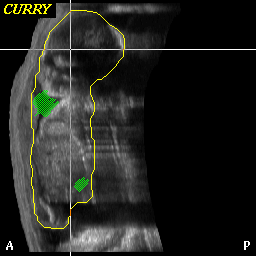
\includegraphics[height=3.5cm, width=3.5cm]{pictures/BA-img1.png}
\vspace{2pt}
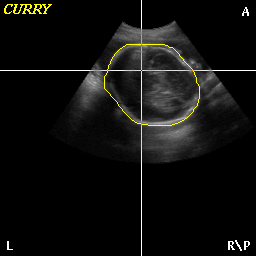
\includegraphics[height=3.5cm, width=3.5cm]{pictures/BA-img2.png}
\vspace{2pt}
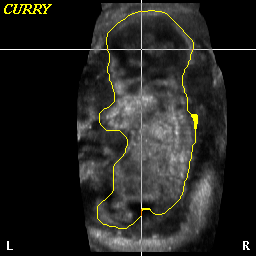
\includegraphics[height=3.5cm, width=3.5cm]{pictures/BA-img3.png}
\caption{Segmentierung (gelb) des F�tus in den verwendeten
Ultraschallbildern mit Pass-Marker (gr�n).}%
%\label{}%
\end{figure}
\end{frame}

\begin{frame}
\frametitle{Randelementediskretisierung}
\begin{figure}%
	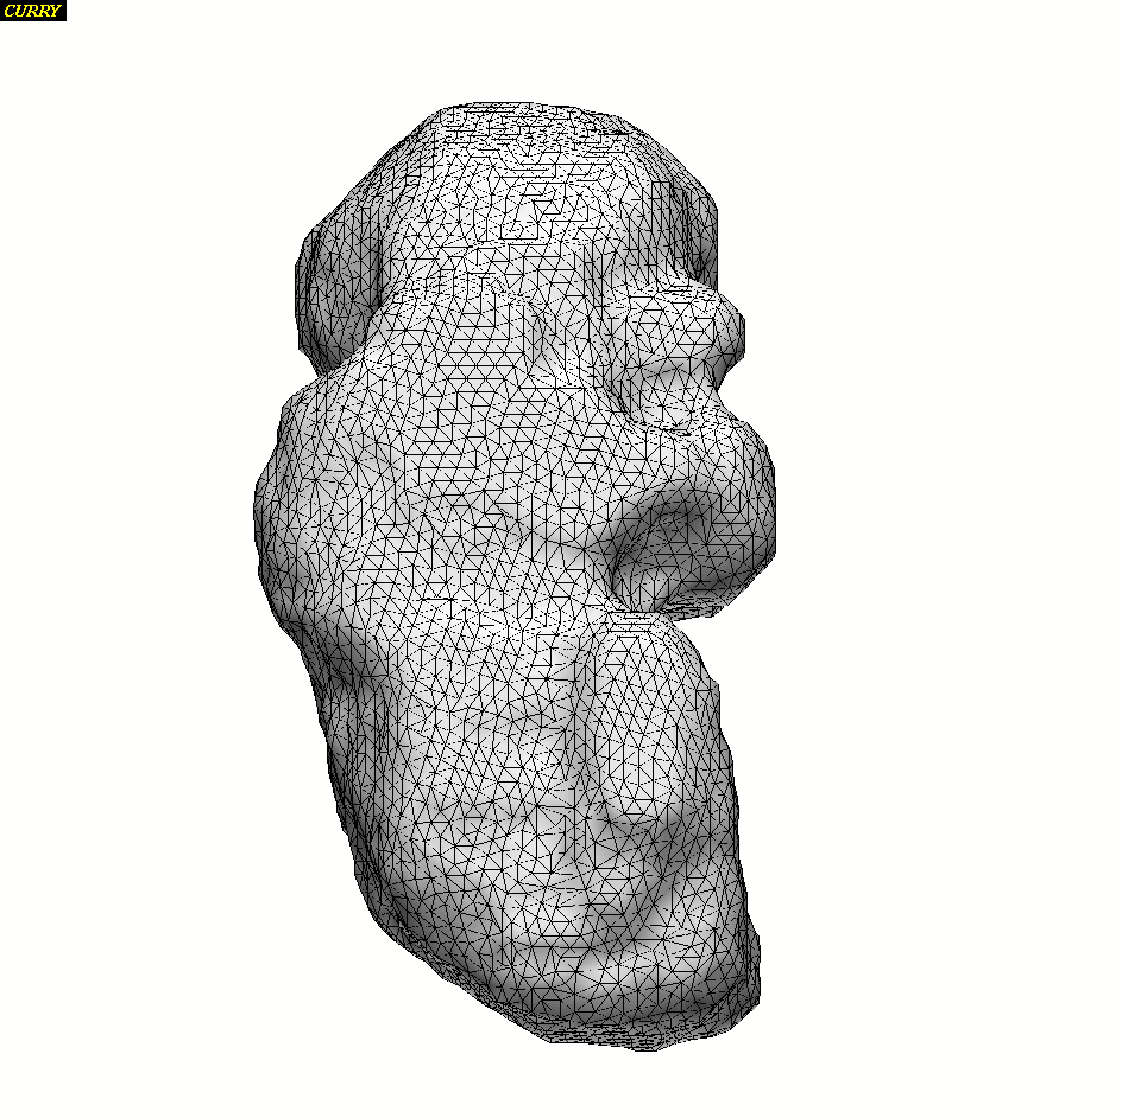
\includegraphics[height=4.5cm]{pictures/BA-img4.pdf}
  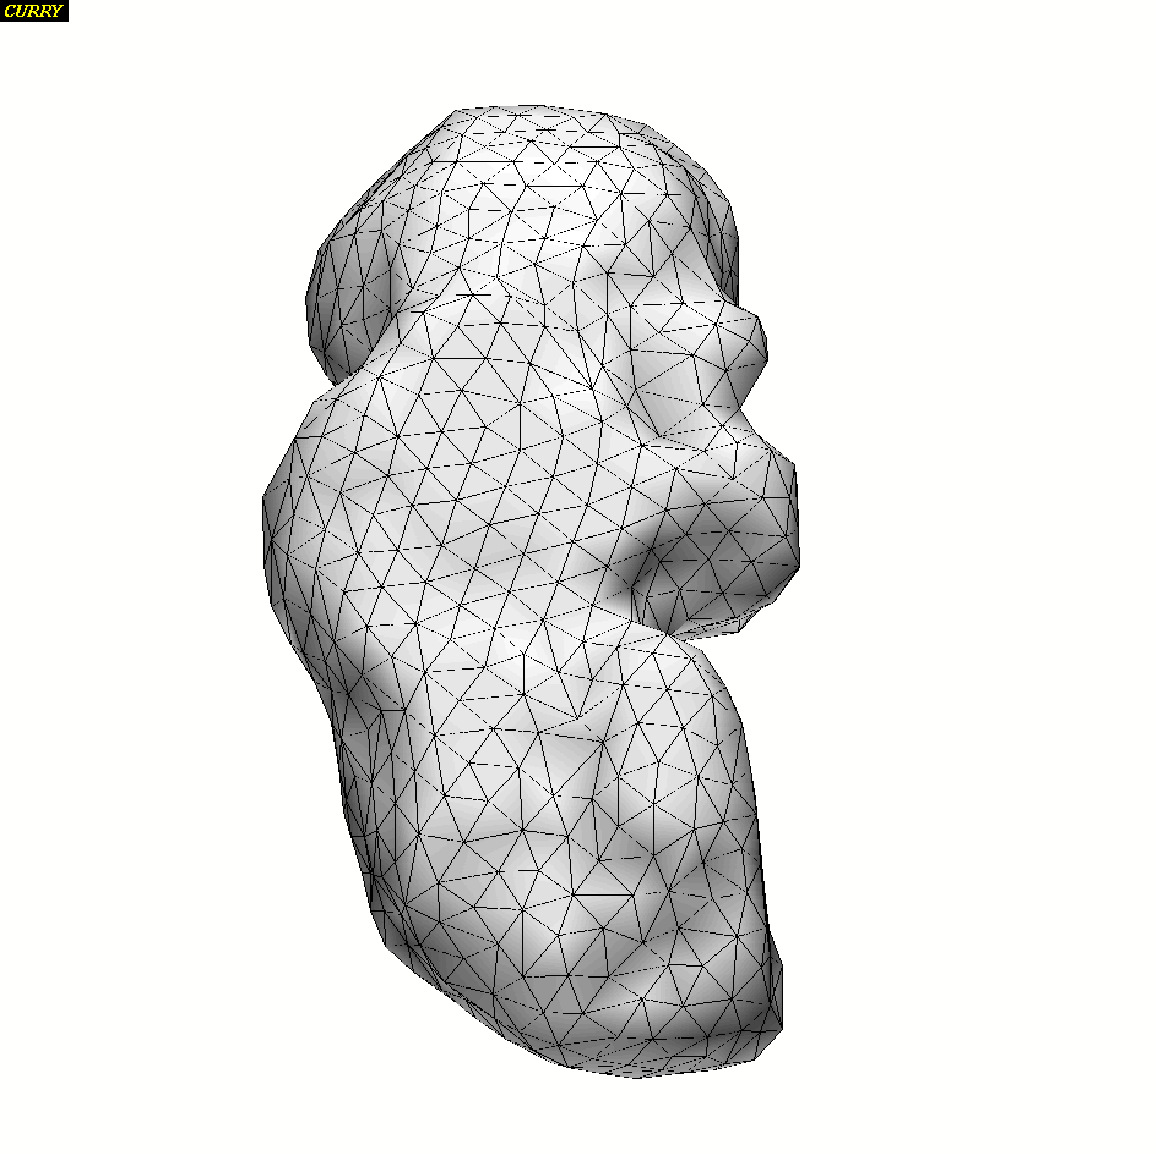
\includegraphics[height=4.5cm]{pictures/BA-img5.pdf}
\caption{Volumenleitermodell des F�tus mit feiner (3mm)
Randelementediskretisierung (links) und grober (9mm, rechts) in frontaler
Ansicht.}%
%\label{}%
\end{figure}
\end{frame}

\begin{frame}
\frametitle{Leitf�higkeit}
%\begin{definition}
	%\begin{itemize}
	%\item 
	Aneinadergrenzende Kompartimente besitzen eine unterschiedliche spezifische elektrische Leitf�higkeit
	%\end{itemize}
%\end{definition}
\begin{example}
\begin{itemize}
	\item Leitf�higkeit des F�tus $\sigma_K = 0.2 \frac{S}{m}$ \cite{a3}
  \item Leitf�higkeit der Vernix caseosa $\sigma_V = 0.000002 \frac{S}{m}$ \cite{a3}%
\end{itemize}
\end{example}
\begin{figure}%
%\includegraphics[height=3cm]{pictures/fetus+vernix.png}
\includegraphics[height=2cm]{pictures/kopf+vernix.png}
\caption{Segmentierungsergebniss f�r F�tuskopf mit Vernix caseosa.}
\end{figure}
\end{frame}

\subsection{Sensorsystem und Quellenmodell}
\begin{frame}
  \frametitle{Virtuelles Sensorsystem}
  \begin{figure}%
  % we can use also: mpeg wmv mpg swf
  \includemovie[poster]{4.5cm}{4.5cm}{multimedia/animation.avi}
  \includegraphics[height=4.5cm]{pictures/1477-044X-2-6-2-l.jpg}
\caption{(links) BEM-Modell ausgehend von der Segmentierung des
F�tus (hautfarben) mit virtuellem SQUID-Sensorsystem
(blau), (rechts) Sensorsystem Argos 200 \cite{15341659}}%
%\label{}%
\end{figure}
\end{frame}

%\subsection{Quellenmodell}
\begin{frame}
\frametitle{Elektrische Dipole}
%\begin{definition}
%    \begin{equation}
%		\mathit{I} = \int_{S}{\vec{J} \cdot \mathit{d}\vec{A}} = \int_{V}{(\nabla \cdot \vec{J})\mathit{d}{V}}
%		\end{equation}
%		\begin{equation}
%		\vec{j} = \int_{l}{I \mathit{d}\vec{l}} = \int_{V}{\vec{J}\mathit{d}{V}}
%		\end{equation}
%\end{definition}
%\begin{itemize}
%	\item[\textit{I}] Stromst�rke
%	\item[\textit{J}] Stromdichte
%	\item[\textit{j}] Elektrisches Dipolmoment (Einheit: $\mu A mm$)
%\end{itemize}
%\begin{theorem}
Als Quellen wurden elektrische Einzeldipole verwendet.
\begin{itemize}
	\item Es wurden �ber 1000 Quellenpositionen im Gehirn des F�tusmodells gleichm��ig verteilt.
	\item F�r die Ausrichtung der Quellen wurden die drei orthogonalen Raumesrichtungen: cranial, dorsal und sinistral gew�hlt
	\item das elektrisches Dipolmoment der Quellen betrug $1 \mu A mm$ (St�rke der Quellen)
\end{itemize}
%Der Dipol besteht aus einer Quelle im Dendriten und einer Senke im Soma.
%\end{theorem}
\end{frame}

\begin{frame}
	\frametitle{Quellenpositionen}
	%Verteilung der Quellen im Gehirnvolumen des F�tusmodells mit definiertem Abstand zur Kopfoberfl�che
	\begin{figure}%
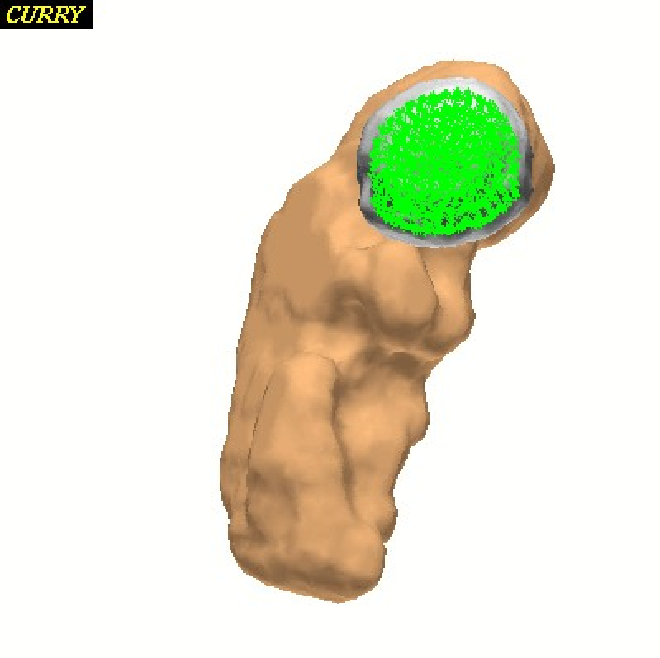
\includegraphics[height=4cm]{pictures/BA-img10.pdf}
\caption{Volumenpunkte (hellgr�n) im
Volumenleitermodell des F�tus (hautfarben) und Kopfes (grau).}%
%\label{}%
\end{figure}
    %\pause
    %\includegraphics[width=5cm,height=5cm]{pictures/1477-044X-4-5-4.jpg}
\end{frame}
\subsection{Variation von Parametern}
\begin{frame}
\frametitle{Randelementediskretisierung}
\begin{itemize}
	%\item Vereinfachung der Oberfl�chen mit Dreiecksnetzen
	%\pause
	\item Variation der Dreiecksseitenl�nge
	\pause
	\item Dreiecksseitenl�ngen beim Abdomen: \textcolor{red}{12 mm}, \textcolor{green}{16 mm}, \textcolor{blue}{20mm} (4-mm-Schritte)
  \pause
	\item Dreiecksseitenl�ngen bei der Vernix caseosa: \textcolor{red}{3 mm}, \textcolor{green}{5 mm}, \textcolor{blue}{7mm, 9mm} (2-mm-Schritte)
  \pause
	\item Dreiecksseitenl�ngen bei der innersten Schicht: \textcolor{red}{3 mm}, \textcolor{green}{5 mm}, \textcolor{blue}{7mm, 9mm} (2-mm-Schritte)
	\pause
	\item Als Referenz wurde das Modell von der F�tussegmentierung mit der feinsten Randelementediskretisierung verwendet.
	\end{itemize}
\end{frame}

\begin{frame}
\frametitle{Segmentierung und Schichtdicke der Vernix caseosa}
\begin{itemize}
	%\item Vereinfachung der Oberfl�chen mit Dreiecksnetzen
	%\pause
	\item Modellierung des gesamten F�tus im Vergleich mit der Modellierung des F�tuskopfes
	\pause
	\item Variation der Schichtdicke der Vernix caseosa von 2 mm bis 4 mm (1-mm-Schritte)
\end{itemize}
\end{frame}

\subsection{Vorw�rtsrechnung und L�sung des inversen Problems}
\begin{frame}
  \frametitle{Vorw�rtsl�sung}
  %\begin{itemize}
			%\item 
			L�sung des direkten Problems f�r definierte Quellenparameter
	%\end{itemize}
	\begin{figure}%
	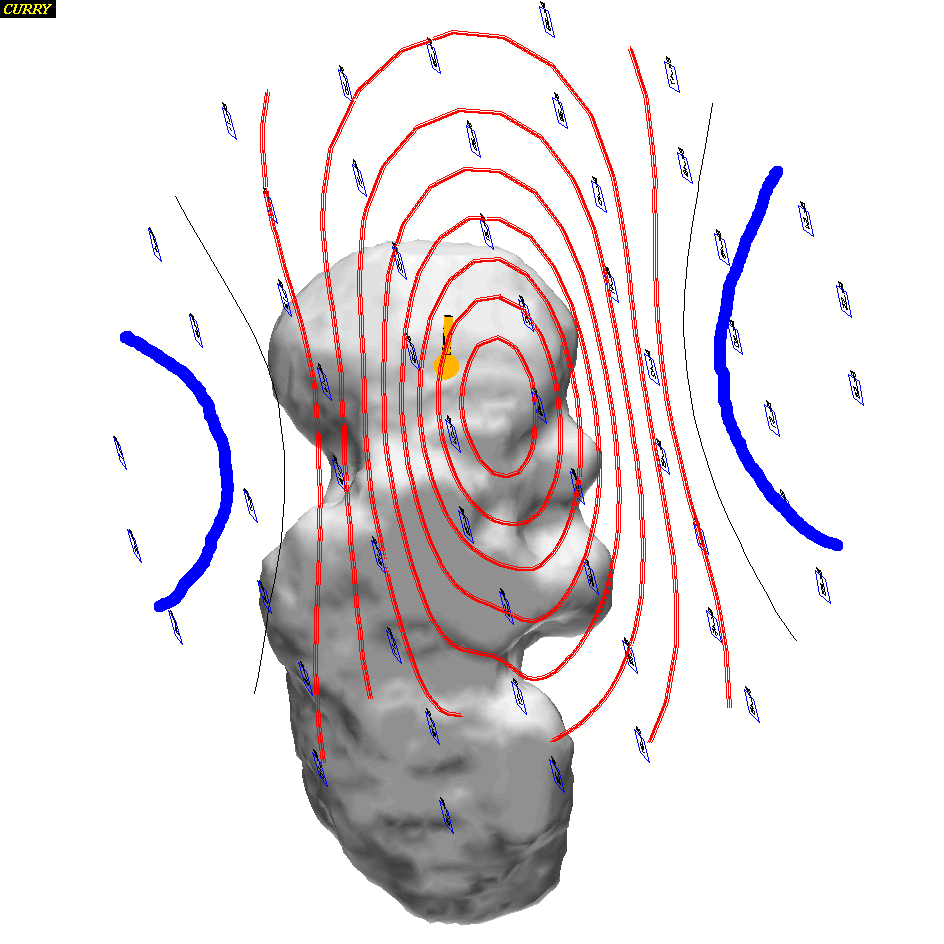
\includegraphics[height=3.5cm, width=3.5cm]{pictures/BA-img11.png}
  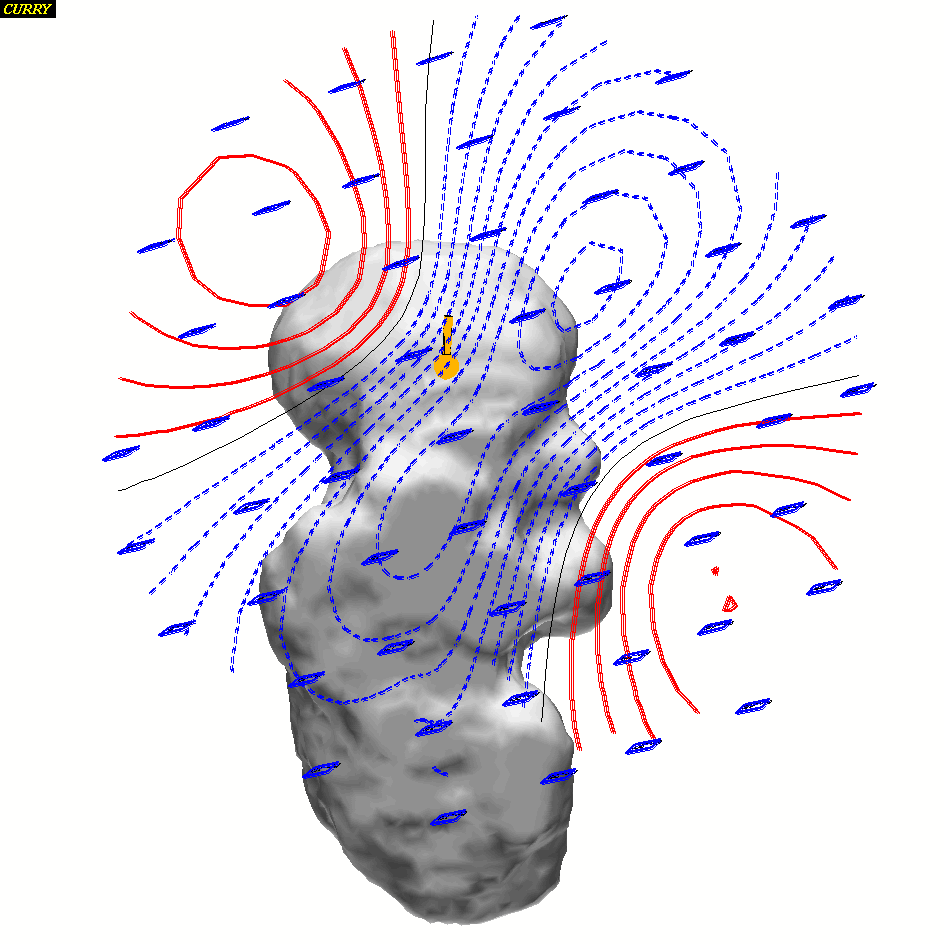
\includegraphics[height=3.5cm, width=3.5cm]{pictures/BA-img12.png}
  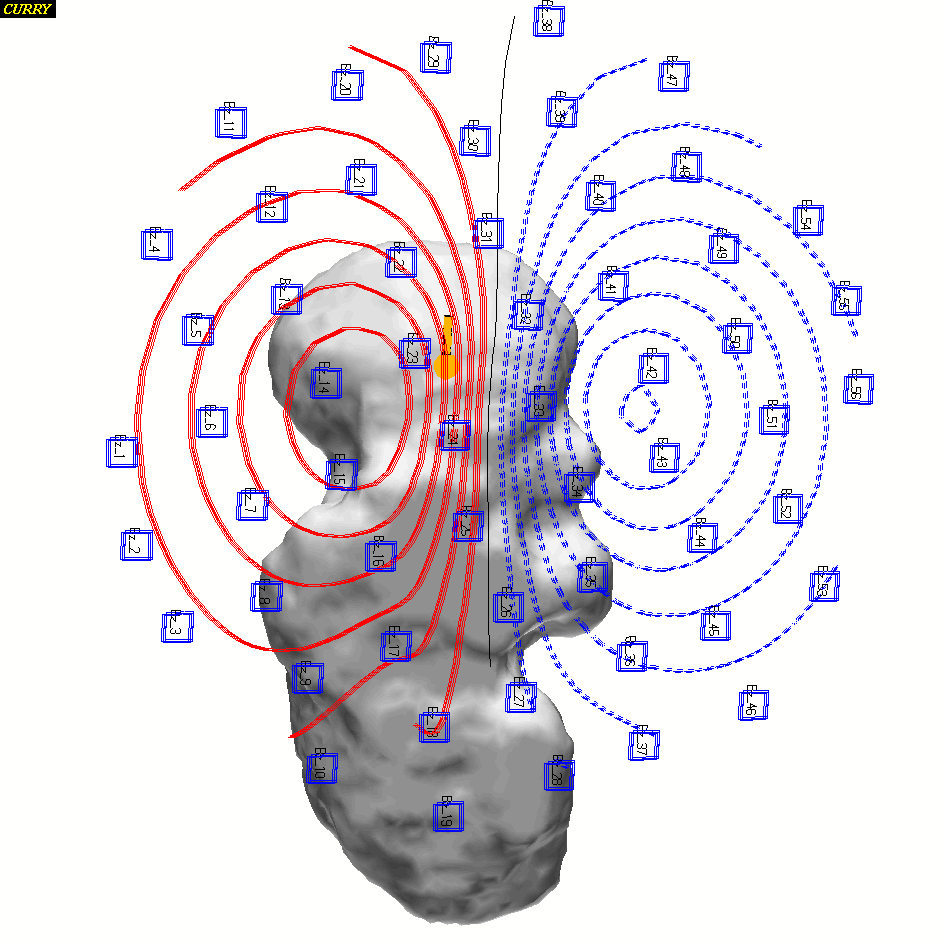
\includegraphics[height=3.5cm, width=3.5cm]{pictures/BA-img13.png}
\caption{Feldbilder einer Simulation mit cranialer
Dipolorientierung im BEM{}-Modell, in den drei Sensorausrichtungen x
(links), y (Mitte) und z (rechts) in frontaler Ansicht.}%
\label{A10}%
\end{figure}
\end{frame}

\begin{frame}
\frametitle{Quellenrekonstruktion}
\begin{itemize}
	%\item Vereinfachung der Oberfl�chen mit Dreiecksnetzen
	%\pause
	\item Vorgabe der bekannten Startpositionen f�r den Simplex-Algorithmus
	\pause
	\item Berechnung der Orientierung und der Amplitude (lineares Problem)
	\end{itemize}
\end{frame}

%\subsubsection{Bewertungskriterien}

\begin{frame}
\frametitle{Bewertung der Vorw�rtsrechnung}
\begin{equation}
\mathit{RDM}=\sqrt{\sum
_{i=1}^{n}\left(\frac{\mathit{meas}_{i}}{\sum
_{j=1}^{n}{\mathit{meas}_{j}^{2}}}-\frac{\mathit{ref}_{i}}{\sum
_{j=1}^{n}{\mathit{ref}_{j}^{2}}}\right)^{2}}
\end{equation}
\begin{equation}
\mathit{MAG}=\sqrt{\frac{\sum
_{i=1}^{n}{\mathit{meas}_{i}^{2}}}{\sum
_{i=1}^{n}{\mathit{ref}_{i}^{2}}}}
\end{equation}
\begin{itemize}
	\item[meas] Messwerte des magnetischen Feldes im Sensorarray
	\item[ref] Werte des Referenzfeldes im Sensorarray
	\item[\textit{RDM}] Relative difference measure, Kenngr��e f�r den Topologiefehler (minimaler Fehler: \textit{RDM}=0)
	\item[\textit{MAG}] Amplitudenfaktor, Gr��e f�r die Amplitudenabweichung (minimaler Fehler: \textit{MAG}=1)
\end{itemize}
\cite{Guellmar2010145}
\end{frame}

\begin{frame}
\frametitle{Bewertung der L�sung des inversen Problems}
\begin{equation}
\alpha =\arccos \left(\frac{\vec{r}\cdot
\vec{s}}{\left|{\vec{r}}\right|\cdot \left|{\vec{s}}\right|}\right)
\end{equation}
\begin{equation}
a=\frac{\left|{\vec{r}}\right|}{\left|{\vec{s}}\right|}
\end{equation}
\begin{itemize}
	\item[$\vec{r}$] Rekonstruiertes Dipolmoment
	\item[$\vec{s}$] Dipolmoment der entsprechenden Simulation
	\item[$\alpha$] Winkelabweichung, G�te der Quellenlokalisation (minimaler Fehler: \textit{RDM}=0�)
	\item[\textit{a}] Amplitudenfaktor, Gr��e f�r die Amplitudenabweichung (minimaler Fehler: \textit{MAG}=1)
\end{itemize}
\cite{Guellmar2010145}
\end{frame}  
\section{Ergebnisse}
\subsection{Einfluss der Segmentierung und Randelementediskretisierung}

\begin{frame}
\begin{itemize}
	\item Anzahl der Dreiecke konvergiert f�r verschiedene Segmentierungen mit steigender Seitenl�nge
\end{itemize}
\begin{figure}
\includegraphics[height=6cm]{pictures/Diagram-img1.pdf}
\end{figure}
\end{frame}

\begin{frame}
\begin{itemize}
	\item Bei der Vorw�rtsrechnung entstehen gr��ere Topologieabweichungen bei gr��eren Randelementen
	\item Ergebnisse h�ngen bei der Kopfmodellierung stark von der Dipolorientierung ab
	\pause
	\item RDMs bei Modellen der Kopfsegmentierung 10 mal gr��er als bei Modellen der F�tussegmentierung
	\pause
	\item Rekonstruierte Dipolorientierung weicht bei der Kopfmodellierung stark von der Referenz ab (�ber 60�)
	\pause
	\item Bei der Kopfmodellierung verbessern sich die Ergebnisse der Quellenrekonstrukion mit gr��eren Randelementen
\end{itemize}
\end{frame}

\begin{frame}
\begin{figure}%
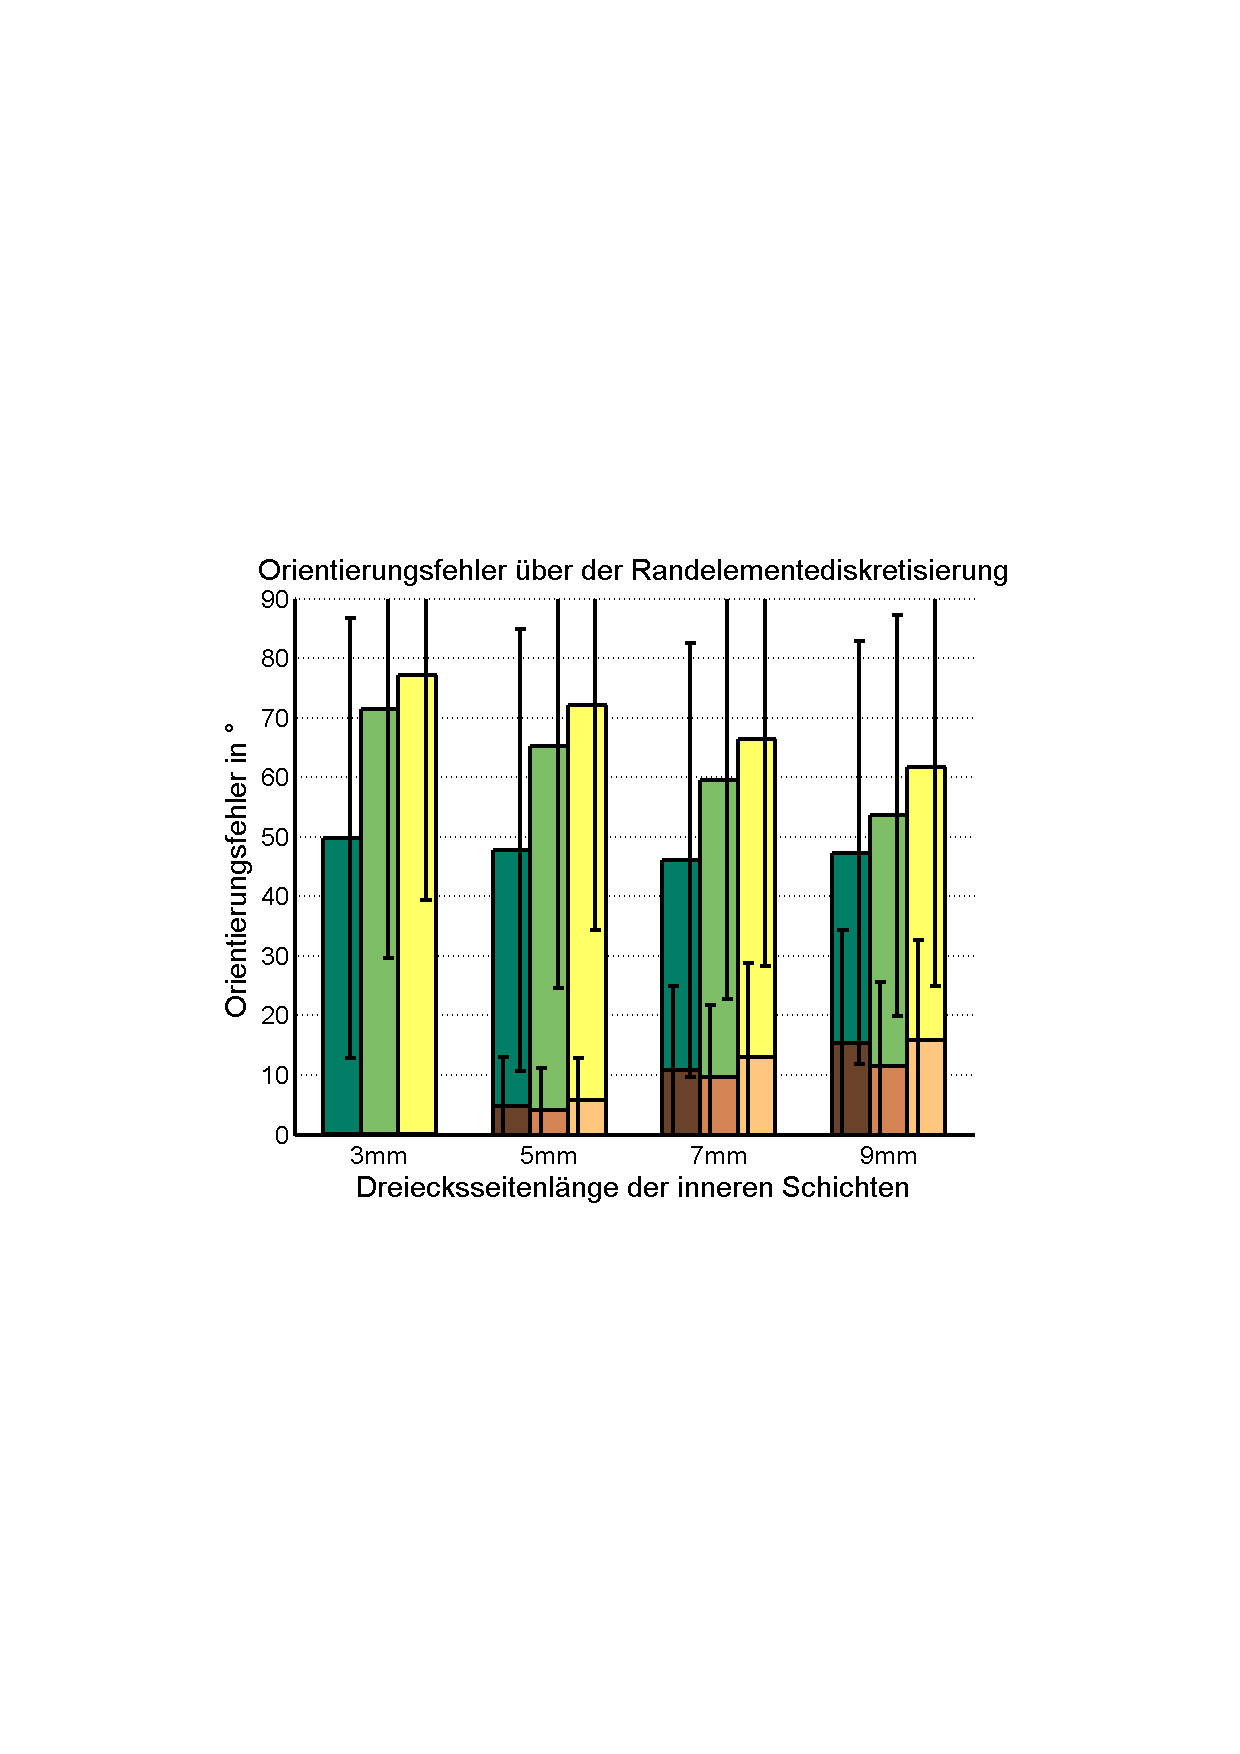
\includegraphics[height=5.5cm]{pictures/BA-img24.png}%
%\caption{}%
%\label{}%
\end{figure}
\begin{center}
\includegraphics[height=1.5cm]{pictures/legend.pdf}
\end{center}
\end{frame}

\subsection{Einfluss der Vernix caseosa}
\begin{frame}
%\frametitle{Variation der Schichtdicke der Vernix caseosa}
\begin{table}%
\caption{\textit{RDM}-Ergebnisse f�r die Dipolorientierungen cranial,
dorsal und sinistral in Abh�ngigkeit von der Schichtdicke der Vernix
caseosa.}%
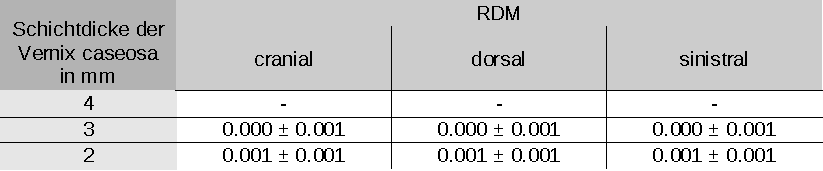
\includegraphics[height=1.7cm]{pictures/BA-img21.pdf}%
%\label{}%
\end{table}
%\begin{figure}%
%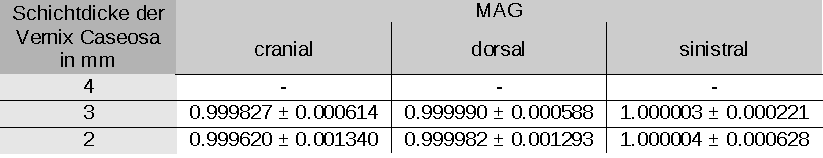
\includegraphics[height=2cm]{pictures/BA-img20.pdf}%
%%\caption{}%
%%\label{}%
%\end{figure}
\begin{table}%
\caption{Winkelabweichungen f�r die Dipolorientierungen
cranial, dorsal und sinistral in Abh�ngigkeit von
der Schichtdicke der Vernix caseosa.}%
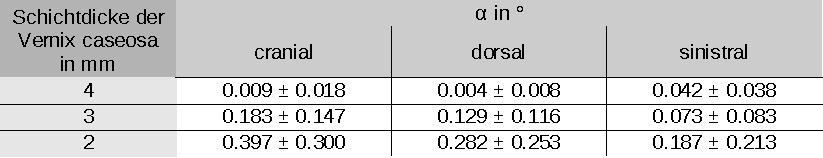
\includegraphics[height=1.7cm]{pictures/BA-img22.pdf}%
%\label{}%
\end{table}
%\begin{figure}
%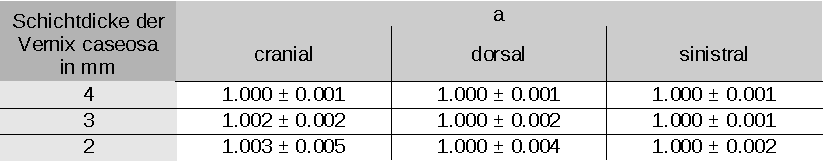
\includegraphics[height=2cm]{pictures/BA-img23.pdf}
%\end{figure}
\end{frame}

\section{Schlussfolgerung und Ausblick}
\begin{frame}
\frametitle{Schlussfolgerungen}
\begin{itemize}
	\item Der Einfluss der Schichtdicke Vernix caseosa ist hier vernachl�ssbar
	\pause
	\item Segmentierung hat gro�en Einfluss auf die Ergebnisse, die Rekonstruktionsergebnisse der Kopfmodellierung sind hier unbrauchbar
	\pause
	%\item �berabtastung der Kopfsegmentierung
	%\item Richtungsabh�ngigkeiten aufgrund der Lage des F�tus im Abdomen
	%\item Ergebnisse sind auf die verwendete Referenz zur�ckzuf�hren
	%\pause
	\item Dreiecksseitenl�nge von 5mm ist ein guter Kompromiss
\end{itemize}
\end{frame}

%\section{Ausblick}
\begin{frame}
\frametitle{Ausblick}
\begin{itemize}
	\item Einsatz von exakteren Modellen (FEM-Modellen) als Referenz
	\pause
	\item Sind die Ergebnisse auf die Qualit�t der US-Bilder zur�ckzuf�hren?
	\pause
	\item Segmentierung/Modellierung aus MRT-Aufnahmen
	\pause
	%\item Lokalisierung des F�tusmodells im Abdomen \cite{0031-9155-52-3-016}
	%\pause
	\item Einfluss von quasisph�rischen Korrekturen \cite{Haueisen1997}
	\pause
	\item Einfluss der Lage des F�tusmodells
	\pause
	\item Untersuchung mit/ohne Vernix caseosa
	\pause
	\item Modellierung des Sch�delknochens
\end{itemize}
\end{frame}
\huge
\begin{frame}
\begin{center}
Vielen Dank f�r ihre Aufmerksamkeit!
\end{center}
\end{frame}
\tiny
\def\newblock{}
\bibliography{Literatur}
\nocite{*} % alle Quellen auff�hren

%  	\input{content/Beamer-Title}
%  	\input{content/Beamer-Content}
%  	\input{content/Beamer-Appendix}

%%%%%%%%%%%%%%%%%%%%%%%%%%%%%%%%%%%%%%%%%%%%%%%%%%%%%%%%%%%%%%%%%%%%%%%
%% Literaturangaben
%%%%%%%%%%%%%%%%%%%%%%%%%%%%%%%%%%%%%%%%%%%%%%%%%%%%%%%%%%%%%%%%%%%%%%%
\end{document}
